\documentclass[11pt]{article}

% Packages
\usepackage[utf8]{inputenc}
\usepackage{amsmath, amssymb, amsthm}
\usepackage{enumitem}
\usepackage{geometry}
\usepackage{fancyhdr}
\usepackage{mathtools}
\usepackage{multicol}
\usepackage[colorlinks=true, urlcolor=blue, linkcolor=blue, citecolor=blue]{hyperref}

% Page layout
\geometry{margin=0.75in}
\pagestyle{fancy}
\fancyhf{}
\rhead{Ian Gallagher}
\lhead{Math 207C Homework}
\rfoot{\thepage}
\setlength{\headheight}{14pt}

% Commands
\newcommand{\vep}{\varepsilon}
\DeclarePairedDelimiter\abs{\lvert}{\rvert}
\newcommand{\norm}[2]{\lVert #1 \rVert_{#2}}

% Environments
\newtheoremstyle{problemstyle}
  {1em} % Space above
  {1em} % Space below
  {\normalfont} % Body font
  {} % Indent amount
  {\bfseries} % Theorem head font
  {} % Punctuation after theorem head
  {\newline} % Space after theorem head
  {} % Theorem head spec

\theoremstyle{problemstyle}
\newtheorem{problem}{Problem}

% Custom commands
\newenvironment{solution}
  {\noindent\textbf{Solution}\quad}
  {\hfill$\blacksquare$\par\vspace{1em}}

% Enumerate styles
\setlist[enumerate,1]{label=(\alph*), ref=\alph*, itemsep=-0.2em, topsep=0.4em}
\setlist[enumerate,2]{label=(\roman*), ref=\roman*, itemsep=0em, topsep=0.2em}

% Title info
\title{Math 258A Challenge \#\texttt{1}}
\author{Ian Gallagher}
\date{\today}

\begin{document}

\maketitle

\section*{Problem 9: Geometry Challenge via Non-linear Optimization Models}
Your challenge is packing $m$ spheres in a box of minimal area. The spheres have a given radius $r_i$, and the problem
is to determine the precise location of the centers $x_i$. The constraints in this problem are that the spheres should
not overlap, and should be contained in a square of center $0$ and half-size $R$. The objective is to minimize the area
of the containing box.
\begin{enumerate}
    \item Show that two spheres of radius $r_1$, $r_2$ and centers $x_1$, $x_2$
        respectively do not intersect if and only if $\|x_1 - x_2\|_2$ exceeds
        a certain number, which you will determine.
    \item Formulate the sphere packing problem as an optimization model. Is the
        formulation you have found convex optimization?
    \item Write (in SCIP, Python, MATLAB, or any other environment) code to
        solve the packing problem of five and six circular disks of the same
        radius inside a square of half-size $R$. What is the optimal size if
        the disks have radius 1?
    \item Do some drawings using MATLAB of the packings you have discovered. Is
        the solution unique?
\end{enumerate}

\begin{solution}
  \newline
  Initial setup of the optimization problem was discussed with both Santiago and Jared. Santiago also assisted with
  debugging a variable bound issue that was forcing all circles to have centers in the first quadrant.
  \begin{enumerate}
    \item\label{part:int} The distance between two spheres is $\norm{x_1 - x_2}{2}$. If we consider the line segment
      connecting the centers of the two spheres, we can see that the spheres do not intersect if and only if the
      distance between their centers is greater than the sum of their radii. Thus, we have:
      \[
        \norm{x_1 - x_2}{2} > r_1 + r_2
      \]
      as the constraint to prevent intersections. If we allow spheres to be tangent at a point then we may relax this
      strict inequality to get
      \[
        \norm{x_1 - x_2}{2} \geq r_1 + r_2
      \]
    \item Our objective is to minimize $R$ subject to the constraints that the spheres don't intersect (discussed in
      part \ref{part:int}) and the constraint that the spheres are entirely contained within the box. The latter condition
      can be restated as $\abs{x_{i, j} \pm r_i} \leq R$ for all $i \in \{1,\dots,m\}, j \in \{1,\dots n\}$ where $n$ is
      the dimension of the space. Putting these together, we have the following minimization problem
      \begin{equation}
        \begin{aligned}
          \min \quad & R \\
          \textrm{s.t.} \quad &  \norm{x_i - x_j}{2} \geq r_i + r_j && \text{ for } i,j \in \{1,\dots,m\}, i \neq r_j \\
                              & \abs{x_{i,j} \pm r_i} \leq R && \text{ for } i \in \{1,\dots,m\}, j \in \{1,\dots,n\}.
        \end{aligned}
      \end{equation}
      This is a non-convex optimization problem. One way to see this is in the case of two circles. If we have two
      placements $x_1, x_2$ of the circles, then linear interpolation of $x_1$ to $x_2$ and vice versa can lead to the
      intersection of the two circles.
    \newpage
    \item I implemented a solver for the given optimization problem using Gurobi. The code can be viewed at the
      following link and is also uploaded along with the writeup:
      \url{https://gist.github.com/iangallagherm/9377faa6099e3c640b34df9183293e41}
      % insert hyperlink below with dummy address
           

      Based on the solutions I found, the minimum half-size $R$ of the box containing the disks is:
      \begin{itemize}
        \item 5 disks: $R \approx 2.4142$
        \item 6 disks: $R \approx 2.6641$
      \end{itemize}
    \item Visualizations of the solution for 5 disks and 6 disks are shown in
      Figures \ref{fig:5disks} and \ref{fig:6disks} respectively. The solution for 6 disks is not unique as it does not
      have a 90 degree rotation symmetry. The solution for 5 disks appears to be unique but I have not verified this.
      % Add figures in 5_circles.png and 6_circles.png
      \begin{figure}[h]
        \centering
        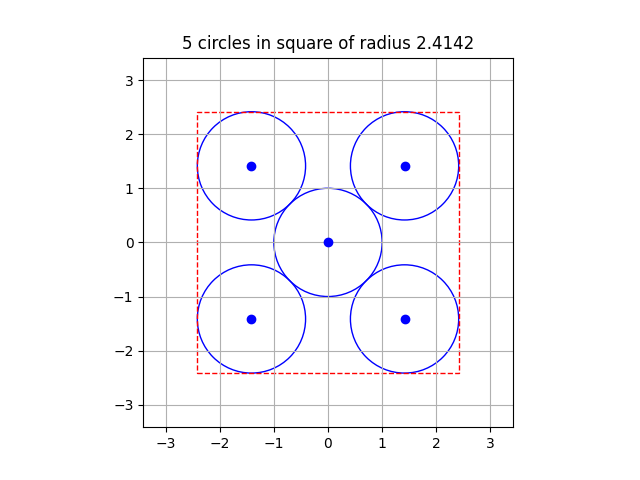
\includegraphics[width=0.5\textwidth]{5_circles.png}
        \caption{Packing of 5 disks}
        \label{fig:5disks}
      \end{figure}

      \begin{figure}[h]
        \centering
        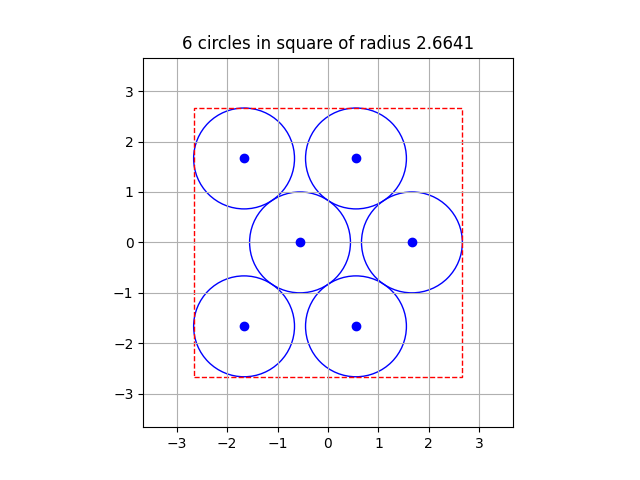
\includegraphics[width=0.5\textwidth]{6_circles.png}
        \caption{Packing of 6 disks}
        \label{fig:6disks}
      \end{figure}
  \end{enumerate}
\end{solution}

\end{document}

